%%%%%%%%%%%%%%%%%%%%%%%%%%%%%%%%%%%%%%%%%%
%%%%%%%%%%%%%                 %%%%%%%%%%%%
%%%%%%%%%%%%%    EXERCISE 1   %%%%%%%%%%%%
%%%%%%%%%%%%%                 %%%%%%%%%%%%
%%%%%%%%%%%%%%%%%%%%%%%%%%%%%%%%%%%%%%%%%%
\begin{exercise}[]{Using the program shown in Figure 1, explain what the output will
    be at LINE A.
    \begin{figure}[ht]
        \centering
        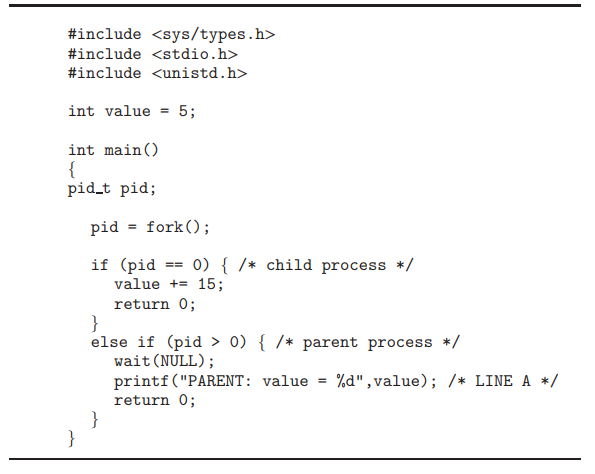
\includegraphics[scale=0.6]{figure 2.png}
        \caption{ What output will be at Line A?}
        \end{figure} }
  \begin{solution}

    The out put will be 5. Although the parent process will wait until the child process finishes executing \texttt{value += 15}, the \texttt{value} in the child process and main process are actually two independent variables. They won't interfere with each other. Therefore, the value of \texttt{value} in the parent process will not be affected and will still be 5 at LINE A.
  \par{~}
  \end{solution}
  \label{ex1}
\end{exercise}


%%%%%%%%%%%%%%%%%%%%%%%%%%%%%%%%%%%%%%%%%%
%%%%%%%%%%%%%                 %%%%%%%%%%%%
%%%%%%%%%%%%%    EXERCISE 2   %%%%%%%%%%%%
%%%%%%%%%%%%%                 %%%%%%%%%%%%
%%%%%%%%%%%%%%%%%%%%%%%%%%%%%%%%%%%%%%%%%%
\begin{exercise}[]{Including the initial parent process, how many processes are created by
    the program shown in Figure 2?
    \begin{figure}[ht]
        \centering
        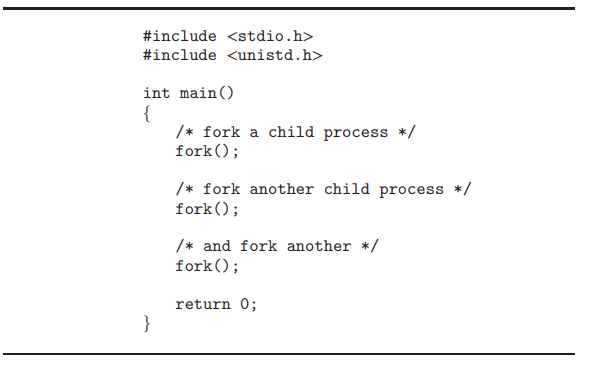
\includegraphics[scale=0.6]{figure 1.png}
        \caption{ How many processes are created?}
        \end{figure} }
  \begin{solution}
    8 processes will be created. Every time \texttt{fork()} is called, the program will be split into two copies of the current executing processes. Therefore, there are $2^3=8$ processes in total.
  \end{solution}
  \label{ex2}
\end{exercise}

%%%%%%%%%%%%%%%%%%%%%%%%%%%%%%%%%%%%%%%%%%
%%%%%%%%%%%%%                 %%%%%%%%%%%%
%%%%%%%%%%%%%    EXERCISE 3   %%%%%%%%%%%%
%%%%%%%%%%%%%                 %%%%%%%%%%%%
%%%%%%%%%%%%%%%%%%%%%%%%%%%%%%%%%%%%%%%%%%
\begin{exercise}[]{Some computer systems provide multiple register sets. Describe what
    happens when a context switch occurs if the new context is already loaded into one of the register sets. What happens if the new context
    is in memory rather than in a register set and all the register sets are in
    use?}
  \begin{solution}
    If the context to be switched to is already in the register sets, the register set pointer will be changed to the present register set. Then an access to the new context registers can be built quickly.

    If the new context is in memory, and all other register sets are occupied, one of the contexts in a register set will be chosen according to certain rules like earliest use or least use. It will be
    moved to memory, and the new context must be loaded from memory
    into the set.
  \end{solution}
  \label{ex3}
\end{exercise}

%%%%%%%%%%%%%%%%%%%%%%%%%%%%%%%%%%%%%%%%%%
%%%%%%%%%%%%%                 %%%%%%%%%%%%
%%%%%%%%%%%%%    EXERCISE 4   %%%%%%%%%%%%
%%%%%%%%%%%%%                 %%%%%%%%%%%%
%%%%%%%%%%%%%%%%%%%%%%%%%%%%%%%%%%%%%%%%%%
\begin{exercise}[]{Describe the actions taken by a kernel to context-switch between processes.}
  \begin{solution}

Context switch refers to the task of switching the CPU core to another process requires performing a state save of the current process and a state restore of a different process.

    Each process is represented in the operating system by a process control block (PCB). A PCB contains many pieces of information associated with a specific process, including process state, program counter, CPU registers, memory-management information, and etc.
    
    When a context switch occurs, the kernel saves the context of the old process in its PCB and loads the saved context of the new process scheduled to run. 
  \end{solution}
  \label{ex4}
\end{exercise}


%%%%%%%%%%%%%%%%%%%%%%%%%%%%%%%%%%%%%%%%%%
%%%%%%%%%%%%%                 %%%%%%%%%%%%
%%%%%%%%%%%%%    EXERCISE 5   %%%%%%%%%%%%
%%%%%%%%%%%%%                 %%%%%%%%%%%%
%%%%%%%%%%%%%%%%%%%%%%%%%%%%%%%%%%%%%%%%%%
\begin{exercise}[]{Explain the role of the init (or systemd) process on UNIX and Linux
    systems in regard to process termination.
    }
  \begin{solution}
    For programs with process relations, if a parent did not invoke \texttt{wait()} and instead terminated, thereby leaving its child processes as orphans. Traditional UNIX systems addressed this scenario by assigning the \texttt{init} process as the new parent to orphan processes.  The \texttt{init} process will periodically invoke \texttt{wait()}, thereby allowing the exit status of any orphaned process to be collected and releasing the orphan’s process identifier and process-table entry.

    In common Linux systems, \texttt{init} has been replaced with \texttt{systemd}, which can still handle such issues in process terminations. In addition, Linux also allows processes other than systemd to inherit orphan processes and manage their termination.
  \end{solution}
  \label{ex5}
\end{exercise}
